%%%%%%%%%%%%%%%%%%%%%%%%%%%%%%%%%%%%%%%%%%%%%%%%%%%%%%%%%%%%%%%%%%
%%%%%%%% ICML 2016 EXAMPLE LATEX SUBMISSION FILE %%%%%%%%%%%%%%%%%
%%%%%%%%%%%%%%%%%%%%%%%%%%%%%%%%%%%%%%%%%%%%%%%%%%%%%%%%%%%%%%%%%%

% Use the following line _only_ if you're still using LaTeX 2.09.
%\documentstyle[icml2016,epsf,natbib]{article}
% If you rely on Latex2e packages, like most moden people use this:
\documentclass{article}

% use Times
\usepackage{times}
% For figures
\usepackage{graphicx} % more modern
%\usepackage{epsfig} % less modern
\usepackage{subfig}
\usepackage{url}
\usepackage{color,graphicx,amsthm,amssymb,amsmath,cite,xspace,setspace}
\usepackage[small,bf]{caption}
\usepackage{multicol, multirow}
\definecolor{orange}{rgb}{.6,0.1,.6}
\newcommand{\rob}[1]{{\textcolor{red}{#1}}}

\usepackage{soul}
\usepackage{algorithm,algorithmic}
\usepackage{colortbl}
\usepackage{rotating}
\usepackage{times}
\usepackage{textcomp}
\usepackage{url}
\usepackage{tabularx}

\usepackage{epsf}
\usepackage{wasysym}
%\usepackage{mdwmath}
\usepackage{mdwtab}

\usepackage{bm}
\usepackage[T1]{fontenc}
\usepackage[font=small,labelfont=bf,tableposition=top]{caption}



\def \bepsilon{\mbox{\boldmath$\epsilon$}}
\def \by{\mbox{\boldmath$y$}}
\def \bx{\mbox{\boldmath$x$}}
% Example definitions.
% --------------------
\def\x{{\mathbf x}}
\def\L{{\cal L}}
\def \ch{c^*}
\def \o{\begin{rotate}{22.5}$\octagon$\end{rotate}}

\def\Rhat{{\widehat R}}
\def\Shat{{\widehat S}}
\def\That{{\widehat T}}
\def\Chat{{\widehat C}}
\def\cT{{\mathcal T}}
\def\cA{{\mathcal A}}
\def\cI{{\mathcal I}}
\def\cS{{\mathcal S}}
\def\cR{{\mathcal R}}
\def\R{{\mathbb R}}
\def\E{{\mathbb E}}
\def \X{{\cal X}}
\def \Y{{\cal Y}}
\def \Z{{\cal Z}}
\def \F{{\cal F}}

\newtheorem{theorem}{Theorem}[section]
\newtheorem{proposition}{Proposition}
\newtheorem{lemma}{Lemma}[section]
\newtheorem{remark}{Remark}
\newtheorem{defNew}{Definition}
\newtheorem{assumption}{Assumption}
\newtheorem{definition}{Definition}
\newtheorem{corollary}{Corollary}[section]
\newtheorem{example}{Example}

\newcommand{\cC}{\mathcal{C}}
\newcommand{\cD}{\mathcal{D}}
\newcommand{\cX}{\mathcal{X}}
\newcommand{\cY}{\mathcal{Y}}
\newcommand{\cU}{\mathcal{U}}
\newcommand{\cE}{\mathcal{E}}
\newcommand{\cP}{\mathcal{P}}
\newcommand{\cM}{\mathcal{M}}
\newcommand{\cZ}{\mathcal{Z}}
\newcommand{\card}[1]{{\vert#1\vert}}
\newcommand{\wh}[1]{{\widehat{#1}}}
\newcommand{\reals}{\mathbb{R}}
\setstcolor{green}
\setul{}{0.3ex}
\def\grad{\nabla}
\def\htheta{{\widehat{\theta}}}
\def\ttheta{{\widetilde{\theta}}}
\def\phtt{{\Phi\htheta_t}}
\def\ttt{\ttheta_t}
\def\hta{\ttheta^{(\alpha)}_{t}}
\def\htb{\ttheta^{(\beta)}_{t}}
\def\hTa{\ttheta^{(\alpha)}_{t+1}}
\def\hTb{\ttheta^{(\beta)}_{t+1}}
\def\tta{\htheta^{(\alpha)}_{t}}
\def\ttb{\htheta^{(\beta)}_{t}}
\def\tTa{\htheta^{(\alpha)}_{t+1}}
\def\tTb{\htheta^{(\beta)}_{t+1}}
\def\bhtheta{\widehat{\btheta}}
\def\bctheta{\widetilde{\btheta}}
\def\btheta{\boldsymbol{\theta}}
\def\bPhi{\boldsymbol{\Phi}}
\def\breg{{D_\psi}}
\def\argmin{\mathop{\!\arg \min}}
\def\deq{{\triangleq}}
\def\sign{\mathop{\mbox{sign}}}
\def \bx{\boldsymbol{x}}
\def \bnu{\boldsymbol{\nu}}
\def \by{\boldsymbol{y}}
\def \bz{\boldsymbol{z}}
\def \bu{\boldsymbol{u}}
\def \bv{\boldsymbol{v}}
\def \bw{\boldsymbol{w}}
\def \bb{\boldsymbol{b}}
\def \bg{\boldsymbol{g}}
\def \ba{\boldsymbol{a}}
\def \bA{\boldsymbol{A}}
\def \bS{\boldsymbol{S}}
\def \bB{\boldsymbol{B}}
\def \bG{\boldsymbol{G}}
\def \bW{\boldsymbol{W}}
\def \bV{\boldsymbol{V}}
\def \bU{\boldsymbol{U}}
\def \bX{\boldsymbol{X}}
\def \bY{\boldsymbol{Y}}
\def \hY{\boldsymbol{\widehat{Y}}}
\def \bC{\boldsymbol{C}}
\def \be{\boldsymbol{\varepsilon}}
\def \bbeta{\boldsymbol{\beta}}
\def\Rhat{{\widehat R}}
\def\Shat{{\widehat S}}
\def\That{{\widehat T}}
\def\Chat{{\widehat C}}
\def\cT{{\mathcal T}}
\def\cA{{\mathcal A}}
\def\cI{{\mathcal I}}
\def\cS{{\mathcal S}}
\def\cR{{\mathcal R}}
\def\R{{\mathbb R}}
\def\E{{\mathbb E}}
\def\P{{\mathbb P}}
\def \X{{\cal X}}
\def \Y{{\cal Y}}
\def \Z{{\cal Z}}
\def \S{{\cal S}}
\def \F{{\cal F}}
\def \K{{\cal K}}
\def \a{{\ast}}
\newcommand{\todo}[1]{{\textcolor{magenta}{#1}}}
\newcommand{\Ave}[1]{\left\langle #1 \right\rangle}
\newcommand{\ave}[1]{\langle #1 \rangle}

\newcommand{\ie}[0]{\emph{i.e., }}
\newcommand{\ea}[0]{\emph{et al. }}
\newcommand{\eg}[0]{\emph{e.g., }}
\newcommand{\cf}[0]{\emph{cf.\ }}
\newcommand{\etc}[0]{\emph{etc.}}



% For citations
\usepackage{natbib}

% For algorithms
\usepackage{algorithm}
\usepackage{algorithmic}

% As of 2011, we use the hyperref package to produce hyperlinks in the
% resulting PDF.  If this breaks your system, please commend out the
% following usepackage line and replace \usepackage{icml2016} with
% \usepackage[nohyperref]{icml2016} above.
\usepackage{hyperref}

% Packages hyperref and algorithmic misbehave sometimes.  We can fix
% this with the following command.
\newcommand{\theHalgorithm}{\arabic{algorithm}}

% Employ the following version of the ``usepackage'' statement for
% submitting the draft version of the paper for review.  This will set
% the note in the first column to ``Under review.  Do not distribute.''
\usepackage[]{icml2016}

% Employ this version of the ``usepackage'' statement after the paper has
% been accepted, when creating the final version.  This will set the
% note in the first column to ``Proceedings of the...''
%\usepackage[accepted]{icml2016}


% The \icmltitle you define below is probably too long as a header.
% Therefore, a short form for the running title is supplied here:
\icmltitlerunning{Learning Representational Brain Networks}

\begin{document}

\twocolumn[
\icmltitle{Learning Representational Brain Networks from fMRI}

% It is OKAY to include author information, even for blind
% submissions: the style file will automatically remove it for you
% unless you've provided the [accepted] option to the icml2016
% package.
\icmlauthor{Urvashi Oswal}{uoswal@wisc.edu}
\icmladdress{Department of Electrical and Computer Engineering, University of Wisconsin-Madison, WI, 53706 USA}

\icmlauthor{Christopher Cox}{crcox@wisc.edu}
\icmladdress{Department of Psychology, University of Wisconsin-Madison, WI, 53706 USA}

\icmlauthor{Matthew A. Lambon Ralph}{matt.lambon-ralph@manchester.ac.uk}
\icmladdress{Neuroscience and Aphasia Research Unit (NARU), School of Psychological Sciences, University of Manchester, Manchester M13 9PL, UK}

\icmlauthor{Timothy T. Rogers}{ttrogers@wisc.edu}
\icmladdress{Department of Psychology, University of Wisconsin-Madison, WI, 53706 USA}

\icmlauthor{Robert Nowak}{nowak@ece.wisc.edu}
\icmladdress{Department of Electrical and Computer Engineering, University of Wisconsin-Madison, WI, 53706 USA}

% You may provide any keywords that you
% find helpful for describing your paper; these are used to populate
% the "keywords" metadata in the PDF but will not be shown in the document
%\icmlkeywords{boring formatting information, machine learning, ICML}

\vskip 0.3in
]

\begin{abstract}
\emph{Representational Similarity Analysis} (RSA) is a tool for discovering brain regions that encode representational similarities among stimuli. Existing RSA methods consider only localized networks, such as specific regions of interest or spherical volumes within cortex.  In this paper we propose a new approach for {\em whole-brain} RSA that can discover arbitrarily structured brain networks (possibly widely distributed and non-local) that encode similarity information.  We pose the RSA problem as a sparsity-regularized multi-task regression problem. This allows us to effectively search over all subsets of voxels (not just localized clusters) to detect similarity-encoding networks.  A baseline approach for this regression task is the group lasso, but this approach may not select important voxels if they happen to be strongly correlated with other voxels.  To address this shortcoming we present a new regularizer for multitask regression with strongly correlated covariates (voxels in fMRI applications) named \emph{Group Ordered Weighted $\ell_1$} (GrOWL).  Theoretically, we show that GrOWL automatically clusters and averages regression coefficients associated with strongly correlated variables. We apply the group lasso and GrOWL approach to whole-brain RSA, demonstrating and comparing our new approach in simulations and real-data experiments.
\end{abstract}

\section{Introduction}
	Network-based approaches to cognitive neuroscience typically assume that mental
representations are encoded as distributed patterns of activation over large neural
populations, with different populations encoding different kinds of representational
structure and communicating this structure to other network components. Extensive research
over the past several years has focused on testing such hypotheses using data from
functional brain imaging techniques such as fMRI. The best-known approach in this vein has
been \emph{Representational Similarity Analysis} (RSA)~\cite{RSA}, which seeks to discover
brain regions whose activity encodes the known psychophysical similarities among some set
of stimuli. RSA is typically applied either to a specific brain region of interest (ROI)
or to many localized regions throughout the brain in process called {\em searchlight
analysis}~\cite{searchlight}. For a given region, RSA computes the cosine distances
between the evoked responses for all stimulus pairs. The resulting neural dissimilarity
matrix is correlated with a target matrix of known psychophysical distances amongst the
stimuli. If these correlations are reliably non-zero, this suggests the corresponding
region may encode the similarity information.

A drawback of ROI and searchlight RSA is that these methods place strong assumptions on
the anatomical structure of the regions thought to encode the similarities of interest
(predefined ROIs or spherical clusters). In this paper we propose a new approach called
{\em Network RSA} that can discover arbitrarily structured brain networks (possibly widely
distributed and non-local) that encode similarity information. The key insight behind our
method is that RSA can be posed as a multi-task regression problem which, in conjunction
with sparsity regularization methods, can automatically detect networks of voxels that
appear to jointly encode similarity information.

Network RSA (NRSA) is summarized as follows (see Sections~\ref{wbrsa1}~and~\ref{wbrsa2}
for further details). Consider a set of $n$ items and suppose we are given an $n \times
n$ similarity matrix $\bS$, where the $ij$-th element $\bS_{ij}$ is the known
psychophysical similarity \cite{similarity} between item $i$ and item $j$. For example,
these may come from human judgments of perceptual similarity between pairs of stimuli.
RSA is based on the hypothesis that there exists a set of voxels whose correlations across
stimuli encode the similarities in $\bS$, as depicted in Figure~\ref{fig.fitting}.

\begin{figure}[!h]
	\centering
    \includegraphics[width=0.5\textwidth]{figures/WRSA.pdf}
  \caption{Representational Similarity Analysis. Traditional RSA methods consider only
    localized brain networks, such as specific regions of interest or spherical clusters
    of the cortex (upper left)~\cite{RSA,searchlight}. We propose a new {\em Network} RSA
    (NRSA) method that can potentially identify non-local brain networks that encode
    similarity information (lower left). Within a set of voxels $\Omega$ (localized or
    non-local), the correlations between the activation patterns resulting from different
    stimuli approximate (perceptual) similarities between the stimuli. } \label{Fig:WRSA}
  \label{fig.fitting}
\end{figure}

Let $\bX \in \R^{n\times p}$ denote a matrix of voxel activations.
Each row corresponds to activations in all $p$ voxels in response to a specific stimulus,
and each column corresponds to the activations in specific voxel to the $n$ different
stimuli. Our generalized notion of RSA, which encompasses conventional ROI \cite{RSA} and
searchlight \cite{searchlight} approaches, involves finding a sparse symmetric positive
semi-definite matrix $\bW\in \R^{p\times p}$ such that

$$\bS \ \approx \bX \bW \bX^T \ .$$

By sparse we mean that at most $k<p$ rows/columns of $\bW$ are nonzero. The locations of
the nonzero elements indicate which voxels are included in the similarity-encoding brain
network, and the weights in $\bW$ indicate the strength of the edges in the network. For
instance, consider the $n\times 1$ activation vectors of two voxels $\bx_k$ and
$\bx_{\ell}$ (i.e., the $k$th and $\ell$th columns of $\bX$). It is easy to show that the
contribution of these two voxels to the similarity representation is given by $ W_{k,\ell}
\, \bx_k \bx_{\ell}^T + W_{\ell,k} \, \bx_\ell \bx_{k}^T$. If $W_{k,\ell}=W_{\ell,k}\neq
0$, then the correlations between the two voxels contribute to the approximation of the
similarity matrix $\bS$. The complete similarity representation can be expressed as
$$\bS \ \approx \ \bX\bW\bX^T \ = \ \sum_{k,\ell=1}^p W_{k,\ell} \, \bx_k \bx_{\ell}^T \ .$$

The approximation problem can be posed as the least squares optimization

$$\min_{\bW} \|\bS-\bX\bW\bX^T\|_F^2 \ , $$

where the objective is the Frobenius norm of the difference between the similarity matrix
$\bS$ and its approximation in terms of voxel activations. Since $\bS$ is a positive
semi-definite matrix, there exists a matrix $\bY$ which satisfies $\bS=\bY\bY^T$ (e.g.,
obtained via eigendecomposition or Cholesky decomposition). Thus, we may instead consider
the optimization

$$\min_{\bB} \|\bY-\bX\bB\|_F^2 \ . $$

For any coefficient matrix $\bB$ the corresponding weight matrix is given by $\bW =
\bB\bB^T$. Both optimizations are convex, but we will work with the latter since it tends
to be easier to solve and also allows us to easily incorporate constraints or
regularizers.

The weight matrix $\bW$ and the coefficient matrix $\bB$ are often expected to exhibit
sparsity and low-rank structure. Indeed, the hypothesis underlying RSA is that a small
subset of the brain encodes the similarity representations, hence the sparsity.
Similarity matrices are often low-rank because of clustering or other relationships
between the items under consideration. For example, in our experimental application
described later in the paper, we find that a rank $r=3$ approximation is quite accurate.
Since the voxel activations represent noisy measurements of brain regions, we also expect
$\bW$ and $\bB$ to be low-rank to encourage clustering in the selected voxels. To account
for this, the optimization above can be modified to obtain sparse and low-rank solutions,
as described next.



\section{Learning Similarity Encodings via Group Lasso}

Consider the group lasso optimization
\begin{equation}\label{eqn.grouplasso}
 \min_{\bB\in \R^{p\times r}} \|\bY-\bX\bB\|_F^2 \ + \ \lambda \|\bB\|_{1,2} \ .
 \end{equation}
Note that the optimization variable $\bB$ is a $p\times r$ matrix, which guarantees a rank
$r$ (or less) solution, and thus similarity representation $\bX\bB\bB^T\bX^T$ will be rank
$r$ at most, which is a simple way to enforce the low-rank constraint. The parameter
$\lambda>0$ is an adjustable weight on the sparsity-promoting regularizer
$\|\bB\|_{1,2}$, which is defined as follows. The rows of $\bB$ are denoted by
$\bbeta_{i\a}$, $i=1,\dots,p$, and the norm
$\|\bB\|_{1,2} \ = \ \sum_{i=1}^n \|\bbeta_{i\a}\|_2$. This encourages solutions with only
a few nonzero rows in $\bB$ \cite{obo11,lounici,vandegeer}.

The main technical innovation in this paper is a new approach to the group lasso that is
designed to cope with strongly correlated covariates (\ie cases in which certain columns
of $\bX$ may be close to, or even exactly, collinear). This is a concern in fMRI, since
certain voxels may have very correlated activation patterns. This problem is illustrated
in Figure~\ref{Fig:sim}, where we simulate a situation where columns $5$ and $7$ of the
data matrix $\bX$ are highly correlated. Group lasso selects one of the corresponding rows
in $\bB$ (row $5$), whereas GrOWL correctly selects both rows $5$ and $7$.

In the standard (single-task) regression problem, this issue has been tackled using many
techniques, including the elastic net \cite{EN}, OSCAR \cite{oscar} and OWL \cite{owl},
and others. We propose a generalization of the recently proposed Ordered Weighted
$\ell_1$ (OWL) approach to the multi-task setting, and thus call our new approach Group
OWL (GrOWL). We show that GrOWL shares many of the desirable features of the OWL method,
namely it automatically clusters and averages regression coefficients associated with
strongly correlated columns of $\bX$. This has two desirable effects, in terms of both
model selection and prediction. First, GrOWL can select all of the relevant voxels in
$\bX$, unlike standard group lasso which may not select relevant voxels if they happen to
be strongly correlated with others. Second, GrOWL encourages the coefficients associated
with strongly correlated voxels to be near or exactly equal. In effect, this averages
strongly correlated voxels which can help to denoise activation patterns and improve
predictions.


\begin{figure}[!t]
    \centering
    \includegraphics[width=0.6\linewidth]{figures/sim3.png}
    \qquad
   \caption{A comparison of group lasso and grOWL optimization solutions with correlated columns in $\bX$ showing that GrOWL selects relevant features (row 5 and 7) even if they happen to be strongly correlated and automatically cluster them by setting the corresponding coefficient rows to be equal (or nearly equal).}
    \label{Fig:sim}
  \end{figure}


	\section{GrOWL}
	\label{Sec:growl}
	
Here we discuss modifications of the group lasso in order to deal with strongly correlated columns in $\bX$.  Our approach is motivated by the recently proposed OWL \cite{owl}, a special case of which is the so-called OSCAR \cite{oscar}.  These methods are designed to automatically cluster and effectively average highly correlated columns in the data matrix, and have been shown to outperform conventional lasso in many applications, particularly in cases of strong correlations. Both OWL and OSCAR deal only with the single regression setting. The main innovation here is the development of new norms, in the spirit of OWL, that allow us to deal with correlated columns in the multiple regression / multitask setting. We define the GrOWL (group OWL) norm, and show that it automatically groups and average highly correlated columns in $\bX$ in the multiple regression setting. 

In this section, we consider the general optimization
\begin{equation}\label{eqn:L1}
\min_{\bB \in \R^{p \times r}} \ L(\bB) \ + \ G(\bB)   
\end{equation}
 where typical loss functions considered here are absolute error, $L(\bB) = \|\bY - \bX \bB \|_1$, or squared Frobenius error, $L(\bB) = \|\bY - \bX \bB \|_F^2$, and $G(\bB)$ is the GrOWL norm defined later in the section. The following results can be extended to the solution of the optimization with squared Frobenius norm loss but, for the sake of simplicity, we consider the absolute error loss in this section (details for extending the theory to Frobenius norm loss are presented in the supplementary material). We give proof sketches for the main theorems and leave the proof details to the supplementary material.  

\subsection{GrOWL penalty}
Let $\bB \in \R^{p\times r}$ and let $\bbeta_{i \a}$ and $\bbeta_{\a  j}$ denote the $i$th row and $j$th column of $\bB$.  Define the GrOWL penalty
\begin{equation}\label{Eqn:growl}
G(\bB) \ =  \sum_{i=1}^p w_i \|\bbeta_{[i]\a}\|_2 , 
\end{equation}
where $\bbeta_{[i]\a}$ is the row of $\bB$ with the $i$-th largest 2-norm and $\bw$ is a vector of non-negative and non-increasing weights.
Before we analyze the GrOWL regularization, we state a generalization of Lemma~2.1 in \cite{owl} which will be useful later in the section. 

\begin{lemma}\label{lemma1}
Consider a vector $\bbeta \in \R^p_+$ and any two of its components $\beta_j$ and $\beta_k$, such that $\beta_j > \beta_k$. Let $\bv \in \R^p_+$ be obtained by applying a transfer of size $\varepsilon, \varepsilon'$ to $\bbeta$ such that $\varepsilon \in (0, (\beta_j - \beta_k )/2]$ and $ -\beta_k \leq \varepsilon' \leq \varepsilon$, that is: $v_j = \beta_j - \varepsilon, v_k = \beta_k + \varepsilon'$, and $v_i = \beta_i$, for $i \neq j, k$. Let $\bw$ be a vector of non-increasing non-negative real values, $w_1 \geq w_2 \geq \cdots \geq w_p \geq 0$, and $\Delta$ be the minimum gap between two consecutive components of vector
$\bw$, that is, $\Delta = \min\{w_i - w_{i+1}, i = 1, \cdots, p - 1\}$. $\Omega_{\bw}(\cdot)$ is the OWL norm with weight vector $\bw$, then
$$\Omega_{\bw}(\bbeta) - \Omega_{\bw}(\bv) \ \geq \ \Delta \varepsilon. \ $$
\end{lemma}

\begin{proof}
The proof is similar to that of Lemma~2.1 in \cite{owl} with different sizes $\varepsilon, \varepsilon'$ and the result follows because we assume that the increase in $k$-th component is less than the decrease in $j$-th component \ie $\varepsilon' \leq \varepsilon$.\\
More intuitively, if $\beta_k$ doesn't go up by $\varepsilon$ in magnitude, then increase its magnitude so that it does and call this $\bv'$ with $v'_j = \beta_j - \varepsilon$ and $v'_k = \beta_k + \varepsilon$.  Then we apply Lemma~2.1 in \cite{owl} to $\bv'$ and $\Omega_{\bw}(\bv) \leq \Omega_{\bw}(\bv')$. 
\end{proof}

The following theorem states that identical variables lead to equal coefficient rows corresponding to those variables in the solution given by the optimization using GrOWL.

\begin{theorem}[Identical columns]\label{ident1}
Let $\widehat \bB$ denote the solution to the optimization in (\ref{eqn:L1}) with $L(\bB) = \|\bY - \bX \bB \|_1$ or $L(\bB) = \|\bY - \bX \bB \|_F^2$.
If columns $\bx_{\a j}$ and $\bx_{\a k}$ satisfy $\bx_{\a j} = \bx_{\a k}$ and the minimum gap, $\Delta > 0$, then
$\widehat \bbeta_{j \a} = \widehat \bbeta_{k \a}$.
\end{theorem}

\textit{Proof sketch.}
The proof is divided into two steps. First, we show $\|\widehat \bbeta_{j \a}\| = \|\widehat \bbeta_{k \a}\|$ and then we further show that the rows are equal. 
We proceed by contradiction. Assume $\|\widehat \bbeta_{j \a}\| \neq \|\widehat \bbeta_{k \a}\|$ and, without loss of generality, suppose $\|\widehat \bbeta_{j \a}\| > \|\widehat \bbeta_{k \a}\|$. We see that there exists a modification of the solution with a smaller GrOWL norm using Lemma~\ref{lemma1} and same data-fitting term, and thus smaller overall objective value which contradicts our assumption that $\widehat \bB$ is the minimizer of $L(\bB) + G(\bB)$. \\

The following theorem states that nearly identical variables lead to equal norm coefficient rows corresponding to those variables in the solution given by the optimization using GrOWL.
\begin{theorem}[Correlated columns 1]\label{thm2}
Let $\widehat \bB$ denote the solution to the optimization in (\ref{eqn:L1}) with $L(\bB) = \|\bY - \bX \bB \|_1$.
If $\bx_{\a j}$ and $\bx_{\a k}$ satisfy $\|\bx_{\a j} - \bx_{\a k}\|_1 \leq \frac{\Delta}{\sqrt{r}} $, then
$\|\widehat \bbeta_{j \a}\| = \|\widehat \bbeta_{k \a}\|$.

\end{theorem}
\textit{Proof sketch.}
The proof is similar to the identical columns theorem. By contradiction and without loss of generality, suppose $\|\widehat \bbeta_{j \a}\| > \|\widehat \bbeta_{k \a}\|$. We show that there exists a transformation of $\widehat{\bB}$ such that the increase in the data fitting term is smaller than the decrease in the GrOWL norm. \\


The following theorem states that nearly identical variables lead to highly correlated coefficient rows corresponding to those variables in the solution given by the optimization using GrOWL.
\begin{theorem}[Correlated columns 2]\label{thm3}
Let $\widehat \bB$ denote the solution to the optimization in (\ref{eqn:L1}) with $L(\bB) = \|\bY - \bX \bB \|_1$.
If $\bx_{\a j}$ and $\bx_{\a k}$ satisfy $\|\bx_{\a j} - \bx_{\a k}\|_1 \leq \frac{\Delta}{\phi\sqrt{r}} $, then
$\|\widehat \bbeta_{j \a} - \widehat \bbeta_{k \a}\| \leq \frac{8\phi \|\widehat \bbeta_{k \a}\|}{4\phi^2+1}$ 
\\which further implies that 
$$1 \geq \frac{\widehat \bbeta_{j \a}^T \widehat \bbeta_{k \a}}{\|\widehat \bbeta_{j \a}\|\| \widehat \bbeta_{k \a}\|} \geq 1 - \frac{1}{2}\left( \frac{8\phi}{4\phi^2+1}\right)^2     \left( \geq 1 - \frac{2}{\phi^2}\right)$$ where $\phi \geq 1$.

\end{theorem}
\textit{Proof sketch.}
By contradiction, suppose $\|\widehat \bbeta_{j \a} - \widehat \bbeta_{k \a}\| \geq \frac{8\phi \|\widehat \bbeta_{k \a}\|}{4\phi^2+1}  \geq \frac{2 \|\widehat \bbeta_{k \a}\|}{\phi}$. We show that there exists a transformation of $\widehat{\bB}$ such that the increase in the data fitting term is smaller than the decrease in the GrOWL norm. This contradicts our assumption that $\widehat{\bB}$ is the minimizer of $L(\bB) + G(\bB)$ and completes the proof.\\

So far, we have seen that the GrOWL penalty has desirable clustering properties that lead to nearly identical coefficient rows. We study two variants of GrOWL with different weight sequences $\bw$. First, we study the weights with linear decay (equivalent to the OSCAR in single-task regression) and call it GrOWL-I. Next, we study the $\ell_1 +\ell_{\infty}$ weight sequence and call it GrOWL-II (see Figure~\ref{Fig:sim}). %We study another variant of the GrOWL which leads to exact clustering of strongly correlated columns. 

%GrOWL-I  :  $w_i = \lambda (p - i) \textnormal{ for } i = 1, \dots,  p $  

%GrOWL-II  :  $w_1 = \lambda_1 +  \lambda_2, w_i = \lambda_1, \textnormal{ for } i = 2, \dots,  p$ 
    




\subsection{Proximal algorithms}
We present computational algorithms for the optimization using the GrOWL norm here. The algorithms rely on the computation of the proximity operator \cite{prox} of the GrOWL norm given by
\begin{eqnarray}\label{proxG}
\textnormal{prox}_{G}(\bV) = \textnormal{arg} \underset{\bB}{ \textnormal{ min } } \frac{1}{2}\|\bB - \bV\|_F^2 + G(\bB) 
\end{eqnarray}
In the following theorem, we solve for the proximity operator of GrOWL in terms of the proximity of OWL. For the exact formulation of $\textnormal{prox}_{\Omega_{\bw}}$, see \cite{candes13}, \cite{ZengFigueiredo2014}.

\begin{theorem} Let $\tilde{v}_i = \| \bv_{i \a}\|$ for $i = 1, \cdots, p$. Then
$\textnormal{prox}_{G}(\bV) = \widehat \bV$, where $i$-th row of $\widehat \bV$ is
\begin{eqnarray}\label{Vhat}
\widehat \bv_{i \a} =  (\textnormal{prox}_{\Omega_{\bw}}(\tilde{\bv}))_i \frac{\bv_{i\a}}{\|\bv_{i \a}\|}
\end{eqnarray}
\end{theorem}
\textit{Proof Sketch:} The proof proceeds by finding a lower bound for the objective function in (\ref{proxG}) and then we show that the proposed solution achieves this lower bound.



\begin{figure}[!t]
    \centering
    \includegraphics[width=0.9\linewidth]{sim3.png}
    \qquad
    \begin{tabular}[b]{ccc}
    \hline
    	GrOWL-I:	& $w_i = \lambda (p - i) \textnormal{ for } i = 1, \dots,  p $   &\\ 
	GrOWL-II:	& $w_1 = \lambda_1 +  \lambda_2, w_i = \lambda_1 \textnormal{ for } i = 2, \dots,  p$  &\\ \hline
    \end{tabular}
    \caption{A comparison of group lasso and grOWL optimization solutions with correlated columns in $\bX$ showing that GrOWL-I and GrOWL-II select relevant features (row 5 and 7) even if they happen to be strongly correlated and automatically cluster them by setting the corresponding coefficient rows to be equal (or nearly equal).}
    \label{Fig:sim}
  \end{figure}



	\section{Network RSA: Simulated Data}
        \label{wbrsa1}
	In this section we illustrate comparative properties of group lasso, GrOWL-I and GrOWL-II
by applying these to the analysis of synthetic data generated from a simple neural network
motivated by the triangle model of word-reading (Figure~\ref{fig.network} top left). This
feed-forward network takes a model analog of word spelling as input (orthographic layer)
and is trained to generate distributed representations of its meaning (semantic layer) and
pronunciation (phonological layer). The network is deep in that mappings from orthography
to phonology, from orthography to semantics, and from semantics to phonology, are all
mediated by one or more hidden layers of units. The model's ability to generate
phonological output is mediated by two separate pathways: a {\em direct} route mediated by
a single hidden layer, and an ``indirect'' route composed of three hidden layers, which
must first compute mappings from orthography to semantics, then project onward to
contribute to the phonological output units.

%On each learning trial the orthographic pattern corresponding to a particular word is
%clamped over input units. Each unit's net input is then computed as the dot product of
%the activations of connected sending units and the values of interconnecting weights.
%Activation values are then taken as a sigmoid function of the unit's net input. Output
%activations generated across semantic and phonological units are compared to target
%values for the corresponding words, and the model is trained with gradient descent to
%reduce the squared error. Training proceeds until all semantic and phonological output
%units are within 0.1 of their target values for all patterns. 

The triangle model provides an interesting test case for discovery of representational
similarity structure, because different kinds of structure emerge through learning in
different network components. The central idea is that orthographic and phonological
similarities are highly systematic: items that are similar in spelling are likely (though
not guaranteed) to be similar in pronunciation. These regularities are easily learned
within the direct pathway mapping from orthography to phonology, allowing the system to
generate appropriate pronunciations for previously unseen word-forms. In contrast, the
relationship between orthographic and semantic similarity structure is unsystematic:
similarity of word spelling does not necessarily predict similarity of meaning. Thus other
pathways within the network, in learning to map from orthography to semantics and from
semantics to phonology, come to encode different similarity relations amongst the
words~\cite{PlautETAL96,HarmSeidenberg04}.

To capture these properties of the triangle framework, we generated model ``orthographic''
word representations in which individual patterns were sampled from 6 overlapping clusters
of binary input features, roughly corresponding to different orthographic neighborhoods.
For each such ``word'', a corresponding ``phonological'' pattern was generated by flipping
each binary feature from the orthographic pattern with probability 0.1. Thus phonological
patterns were distorted variants of the orthographic patterns, creating high systematicity
between these. Finally, for each word we also created a semantic pattern by generating a
set of binary semantic features also organized into clusters. Across items, these vectors
expressed a hierarchical similarity structure with two broad superordinate clusters each
composed of three tighter clusters. Importantly, the similarity structure expressed by the
semantic vectors was independent of the structure expressed in the
orthographic/phonological patterns. 

The left bottom panel in Figure~\ref{fig.network} shows, for each layer of one trained
model, the cosine distances encoded amongst the 30 model ``words''. Just from inspection
it is clear that units in the direct pathway from orthography to phonology all encode
roughly the same distances amongst items, reflecting the high systematicity between
orthographic and phonological similarity structure. The semantic layer encodes a very
different set of distances amongst the items while, again from inspection, two of the
three hidden layers in the indirect pathway encode weaker versions of this structure.
Finally the first hidden layer between orthography and semantics appears to encode a blend
of the orthographic and semantic distances. Thus the different components of this simple
word-reading network contribute differentially to the encoding of semantic versus
ortho-phonological similarity structure. 

To create synthetic ``brain imaging data'' we trained 5 models with different initial
weights, corresponding to 5 model subjects. We then presented each trained model with all
30 orthographic inputs and generated a vector of unit activations for each input over the
100 model units. To ensure a high degree of redundancy within our synthetic dataset, this
vector was next concatenated 5 times and then perturbed with independent noise, yielding
measurements from 500 model ``voxels'' in each of 5 different ``subjects''. We then
applied group lasso and GrOWL to find the voxel subsets that encode the targeted semantic
or phonological distances (derived from the target values for the semantic and
phonological output layers of the network). 

We fit statistical models by searching a two-dimensional grid of parameters
($\lambda$, $\lambda_1$), including $\lambda_1=0$ as the special case of GrOWL that is
group lasso. At each grid point we computed the number of ``voxels'' selected (\ie having
non-zero weights). We assessed how well each fitted model identified the ``voxels'' that
encode phonological structure (all those along the direct pathway) and those that encode
semantic structure (the semantic layer itself and the middle layer and third hidden layer
in the indirect pathway) by computing hit rates and false alarm rates. Figure~\ref{fig.roc}
shows these data for group lasso and GrOWL. All three models show relatively low and
equivalent cross-validation error; however GrOWL-II achieves this error rate while
selecting considerably more voxels. The ROC plots in Figure~\ref{fig.roc} further show
that GrOWL-II is not just selecting additional voxels at random: its ability to
discriminate signal-carrying from non-signal carrying voxels outstrips the group lasso
considerably.

The right panel of Figure~\ref{fig.network} show the frequency with which each model unit
is selected for the best-performing solution in group lasso and GrOWL, in decoding
phonological and semantic similarity. While each method hones in on approximately the
correct subset of network units, the strong sparsity enforced by group lasso is clearly
apparent: target units are much less consistently selected. GrOWL, in contrast,
consistently discovers much more of the signal.

Finally, we considered the ability of GrOWL to reveal the network structure encoding each
kind of similarity, treating the weights in the matrix $\bW$ as direct estimates of the
joint participation of pairs of units in expressing the target similarity. The rightmost
plots of Figure~\ref{fig.network} shows the estimated connectivity, thresholded to show
the 25\% of the non-zero weights with the largest magnitudes. The detected edges clearly
express the network representational substructure: units in the direct pathway are shown
as highly interconnected with one another and weakly or disconnected from those in the
indirect pathway, and vice versa. Thus the search for different kinds of similarity
reveals different functional subnetworks in the model.

\begin{figure*}[!t]
\centering
\includegraphics[width=0.99\textwidth]{figures/Network_results1.png}
\caption{Left panel: Network architecture (top) and the similarity structure expressed in
  each layer (bottom). Red background shows the direct pathway and blue the indirect
  pathway from orthography to phonology. Layers in the two pathways encode different
  similarity structures. The target similarity matrices for the analysis express either
  the semantic structure (top layer) or the phonological structure (bottom right layer).
  Arrows indicate feed-forward connectivity. Right panel: Units selected by group LASSO
  (right) and GrOWL (middle) when decoding semantic (top) or phonological (bottom)
  structure. Colors show the proportion of times across subjects and unit concatenations
  that the unit received a non-zero weight, with red indicating 1 and gray 0. The
  rightmost plots show the largest weights in the associated matrix W for each GrOWL
  model, which pick out two subnetworks in the model.}
\label{fig.network}
\end{figure*}  

\begin{figure*}[!h]
\centering
\subfloat[]{\includegraphics[width=0.4\textwidth]{figures/ROC_sem.pdf}
\label{fig_first_case}}
\hfil
\subfloat[]{\includegraphics[width=0.39\textwidth]{figures/ROC_phon.pdf}
\label{fig_second_case}}
\caption{ROC curves generated by sweeping through $\lambda$ values (for $\lambda = 0$, all
  units are selected and as $\lambda$ is increased fewer units are given non-zero weight).
  Each curve represents a fixed value of $\lambda_1$, where the curve $\lambda_1 = 0$
  corresponds to group lasso. ROC curves are averaged across participants for each method,
  considering both similarity structures, Semantics (left panel) and Phonology (right
  panel).}
\label{fig.roc}
\end{figure*}


	\section{Network RSA: Real Data}
        \label{wbrsa2}
	We will now apply group lasso and GrOWL to the discovery of similarity structure in
whole-brain patterns of neural activity. As with the well-known searchlight RSA (\cite{RSA},
\cite{similarity}), the structue of interest is the set of pairwise similarities among $n$ 
stimuli which is estimated indpendently of the neural data. We compute a rank-$r$
approximation of the $n-by-n$ similarity matrix $\bS = \bY \bY^T$. This is the target $\bY
\in \R^{n \times r} $ matrix for the sparse regression analysis. Participants
perform a cognitive task involving these stimuli while their brains are monitored with
fMRI, which will yield a whole-brain scan every 2 seconds with 3mm cubic resolution. Each
cube is refered to as a voxel. Each voxel contains a timeseries of data, and each time
series can be modeled to estimate how each voxel responds to each stimulus. These estimates
for each of $n$ stimuli and $d$ voxels will be used as the features for modeling the
similarity structure. Because we do not want to presume which of the features jointly
encode the target similarity structure, we will include all voxels that correspond to grey
matter (cerebral cortex) in our analyses.

The model is fit to optimize the object functions specified in (\ref{eqn.grouplasso}) for
group lasso and (\ref{eqn:L1}) for GrOWL. The regularization parameter is selected through
cross-validation, and a final model is fit with that parameter and used to predict the
similarities existing among a set of items in an independent hold-out set. Model
predictions are evaluated by permutation test. The $n$ rows within each of the $r$ columns
of $\bY$ are shuffled independently 1000 times, and the model is refit to each of these
permuted target structures. This maintains all qualities of the original analysis and data,
except that permuted versions of $bY$ are devoid of structure. If the accuracy of the true
model is larger than 97.5\% of the permuted results (corresponding to 2-tailed p<0.05), we
will conclude that the model has discovered voxel subsets that jointly encode some of the
target similarity structure. Moreover, because the model is constrained to be sparse, most
voxels will receive coefficients of zero. Voxels with non-zero coefficients can be
considered important to representing the target similarity structure.

The current experiment aims to answer four questions. (1) Does either approach learn a
model from whole-brain fMRI that can accurately predict the pairwise similarities among
stimuli? (2) Does group lasso or GrOWL learn a more accurate model? (3) Do the fitted
models identify voxels in areas that are consistent with what is known about neural
representations? (4) Do the discovered networks differ when modeling different kinds of
stimilarity structure among the same items?

To answer these questions, we applied both NRSA approaches to discover voxels that
encode the visual or semantic similarity among a set of 37 line drawings of common objects.
We chose this task and set of stimuli because (a) there exist well-understood methods for
objectively measuring the degree of visual similarity among such items \cite{antani02},
(b) it is well known that visual similarity is encoded by neural responses in occipital
and posterior temporal cortices, (c) there are well established feature-norming datasets
that permit validated estimates of semantic similarity, and (d) semantic similarity is
expected to be encoded by different areas than encode visual similarity in the brain.

\subsection{fMRI dataset} The data were collected as part of a larger study from 23
participants at the University of Manchester who were compensated for their time. Each
participant viewed a series of line drawings depicting common objects while their brains
were scanned with fMRI. The line drawings included 37 items, each repeated 4 times for a
total of 148 unique stimulus events. At each trial participants pressed a button to
indicate whether the item could fit in a ``wheely bin'' (a form of trash can common in the
UK).  Scans were collected in a sparse event-related design and underwent standard
pre-processing to align functional images to the anatomy and to remove movement and scanner
artifact and temporal drift. Responses to each stimulus event were estimated at each voxel
using a deconvolution procedure with a standard HRF kernel. For each participant a cortical
surface mask was generated based on T1-weighted anatomical images, and functional data were
filtered to exclude non-cortical voxels. Voxels with estimated responses more than 5
standard deviations from the mean response across voxels were excluded from the analysis.
10k-15k voxels were selected for each participant, and neural responses across all voxels
for each of 148 stimulus events were entered into the analysis. The mean response across
the 4 repeated observations of each item were taken to give 37 item responses for each
participant. Each column corresponding to a voxel was normalized to be of standard
deviation equal to one and a column of ones was added.

\subsubsection*{Target similarities}
\subsubsubsection*{visual}<++>
 Each stimulus was a bitmap of a black-and-white line drawing. We took pairwise Chamfer distance as a proxy for inter-item visual dissimilarities. r = 3 is the smallest value to attain $\|\bS - \bY\bY^T\|_F \leq 0.2$. This $37 \times 3$ matrix $\bY$ was used as the target matrix for the analysis.

\subsubsubsection*{semantic}<++>
Each image depicted a easily namable object, and these names were used to look up feature
norms in the XXX database. The database is a word by feature matrix, where each feature is
something like ``has wings'' or ``can swim''. Each row is populated with the number of
times each feature is listed for that word. The target matrix is derived as the cosine
distance among the vectors for each of the 37 names.

\subsubsection*{Model fitting} For each participant, training data were divided into 9
subsets containing 4--5 stimulus events each. One subset was selected as a final hold-out
set. Models were then fit at each of 10 increasing values of $\lambda$ using 8-fold cross
validation. At each fold we assessed the model using the Frobenius norm of the difference
between the target $\bY$ entries and the predicted $\hY = \bX\widehat{\bB}$ entries for
hold-out items (henceforth the model error). We selected the $\lambda$ with the lowest mean
error for each subject subjects, then fit a full model for each subject at this value and
assessed it against the final hold-out set, considering the model error on hold-out items.
We repeat this process for 9 different final hold-out sets.

\subsection{Results}
%The model cross-validation error at each value of $\lambda$, for both group lasso and GrOWL are recorded and the $\lambda$ corresponding to the minimum error  is recorded. %Note that, with no signal in the data, the expected error is 1. The curves show a U-shape with a minimum at XX, and are clearly less than 1. Thus both approaches appear to be generating better predictions for hold-out items than would be expected from random data. 

Figure \ref{fig.error}(a) shows performance on the final hold-out sets for each
participant, method, and target structure, considering error between predicted ($\bY_z$)
and actual dissimilarities ($\bY$). Both approaches show significantly non-random
prediction. As in our simulations, the GrOWL shows somewhat better performance (lower
error, higher correlation) though all methods show comparable prediction error. We also
note that, as in the simulations, GrOWL selected almost double the number of voxels in each
participant. 

Figure \ref{fig.error}(b) shows the locations of selected voxels (i.e., those with non-zero
coefficients) across all 23 participants for a single cross validation attempt, mapped into a common anatomical space with 4mm
full-width-half-max spatial smoothing and projected onto a model of the cortical surface.
Both methods pick voxels prominently in the occipital and posterior temporal cortices when
modeling visual structure, but in higher-order visual regions associated with object
processing when modeling the semantic structure. This demonstrates that NRSA is sensitive
to the structure being models and that different brain networks feature prominently in
simple visual and higher-level semantic representations. We also see that GrOWL
picks consistently more voxels than group lasso.

Finally, Figure \ref{fig.NW} shows the largest magnitude edges in the $\bW$ matrix for the
best-performing parameterization of group LASSO (top) and GrOWL (bottom) modeling visual
structure in one subject.
Two observations are of note. First, both methods uncover a similar network structure, with
many interconnections in visual cortical regions and some edges connecting to anterior
regions in frontal and temporal cortex. Second, as in the simulations, GrOWL reveals a
much denser network. The results suggest the possibility that subregions of frontal and
temporal cortex may, together with occipeto-temporal cortex, participate in networks that
serve to encode visual similarity structure.

\begin{figure*}[!t]
\centering
\subfloat[]{\includegraphics[width=0.3\textwidth]{figures/Final_Error_Visual.png}
\label{fig_first_case}}
\hfil
\subfloat[]{\includegraphics[width=0.6\textwidth]{figures/brain_final.png}
\label{fig_second_case}}
\caption{Panel (a) shows mean hold-out prediction error for group lasso and GrOWLs for 23 subjects. Panel (b) shows surface maps corresponding to group lasso (left), GrOWL-I (middle) and GrOWL (right) showing the voxels selected for \textit{at least five} and \textit{all nine} cross-validations in the top and bottom rows respectively. The heat map shows the number of subjects for which those voxels were picked. Blue is the least (1 subject) and red is the most (10 or more subjects).}
\label{fig.error}
\end{figure*}

\begin{figure}[!t]
\centering
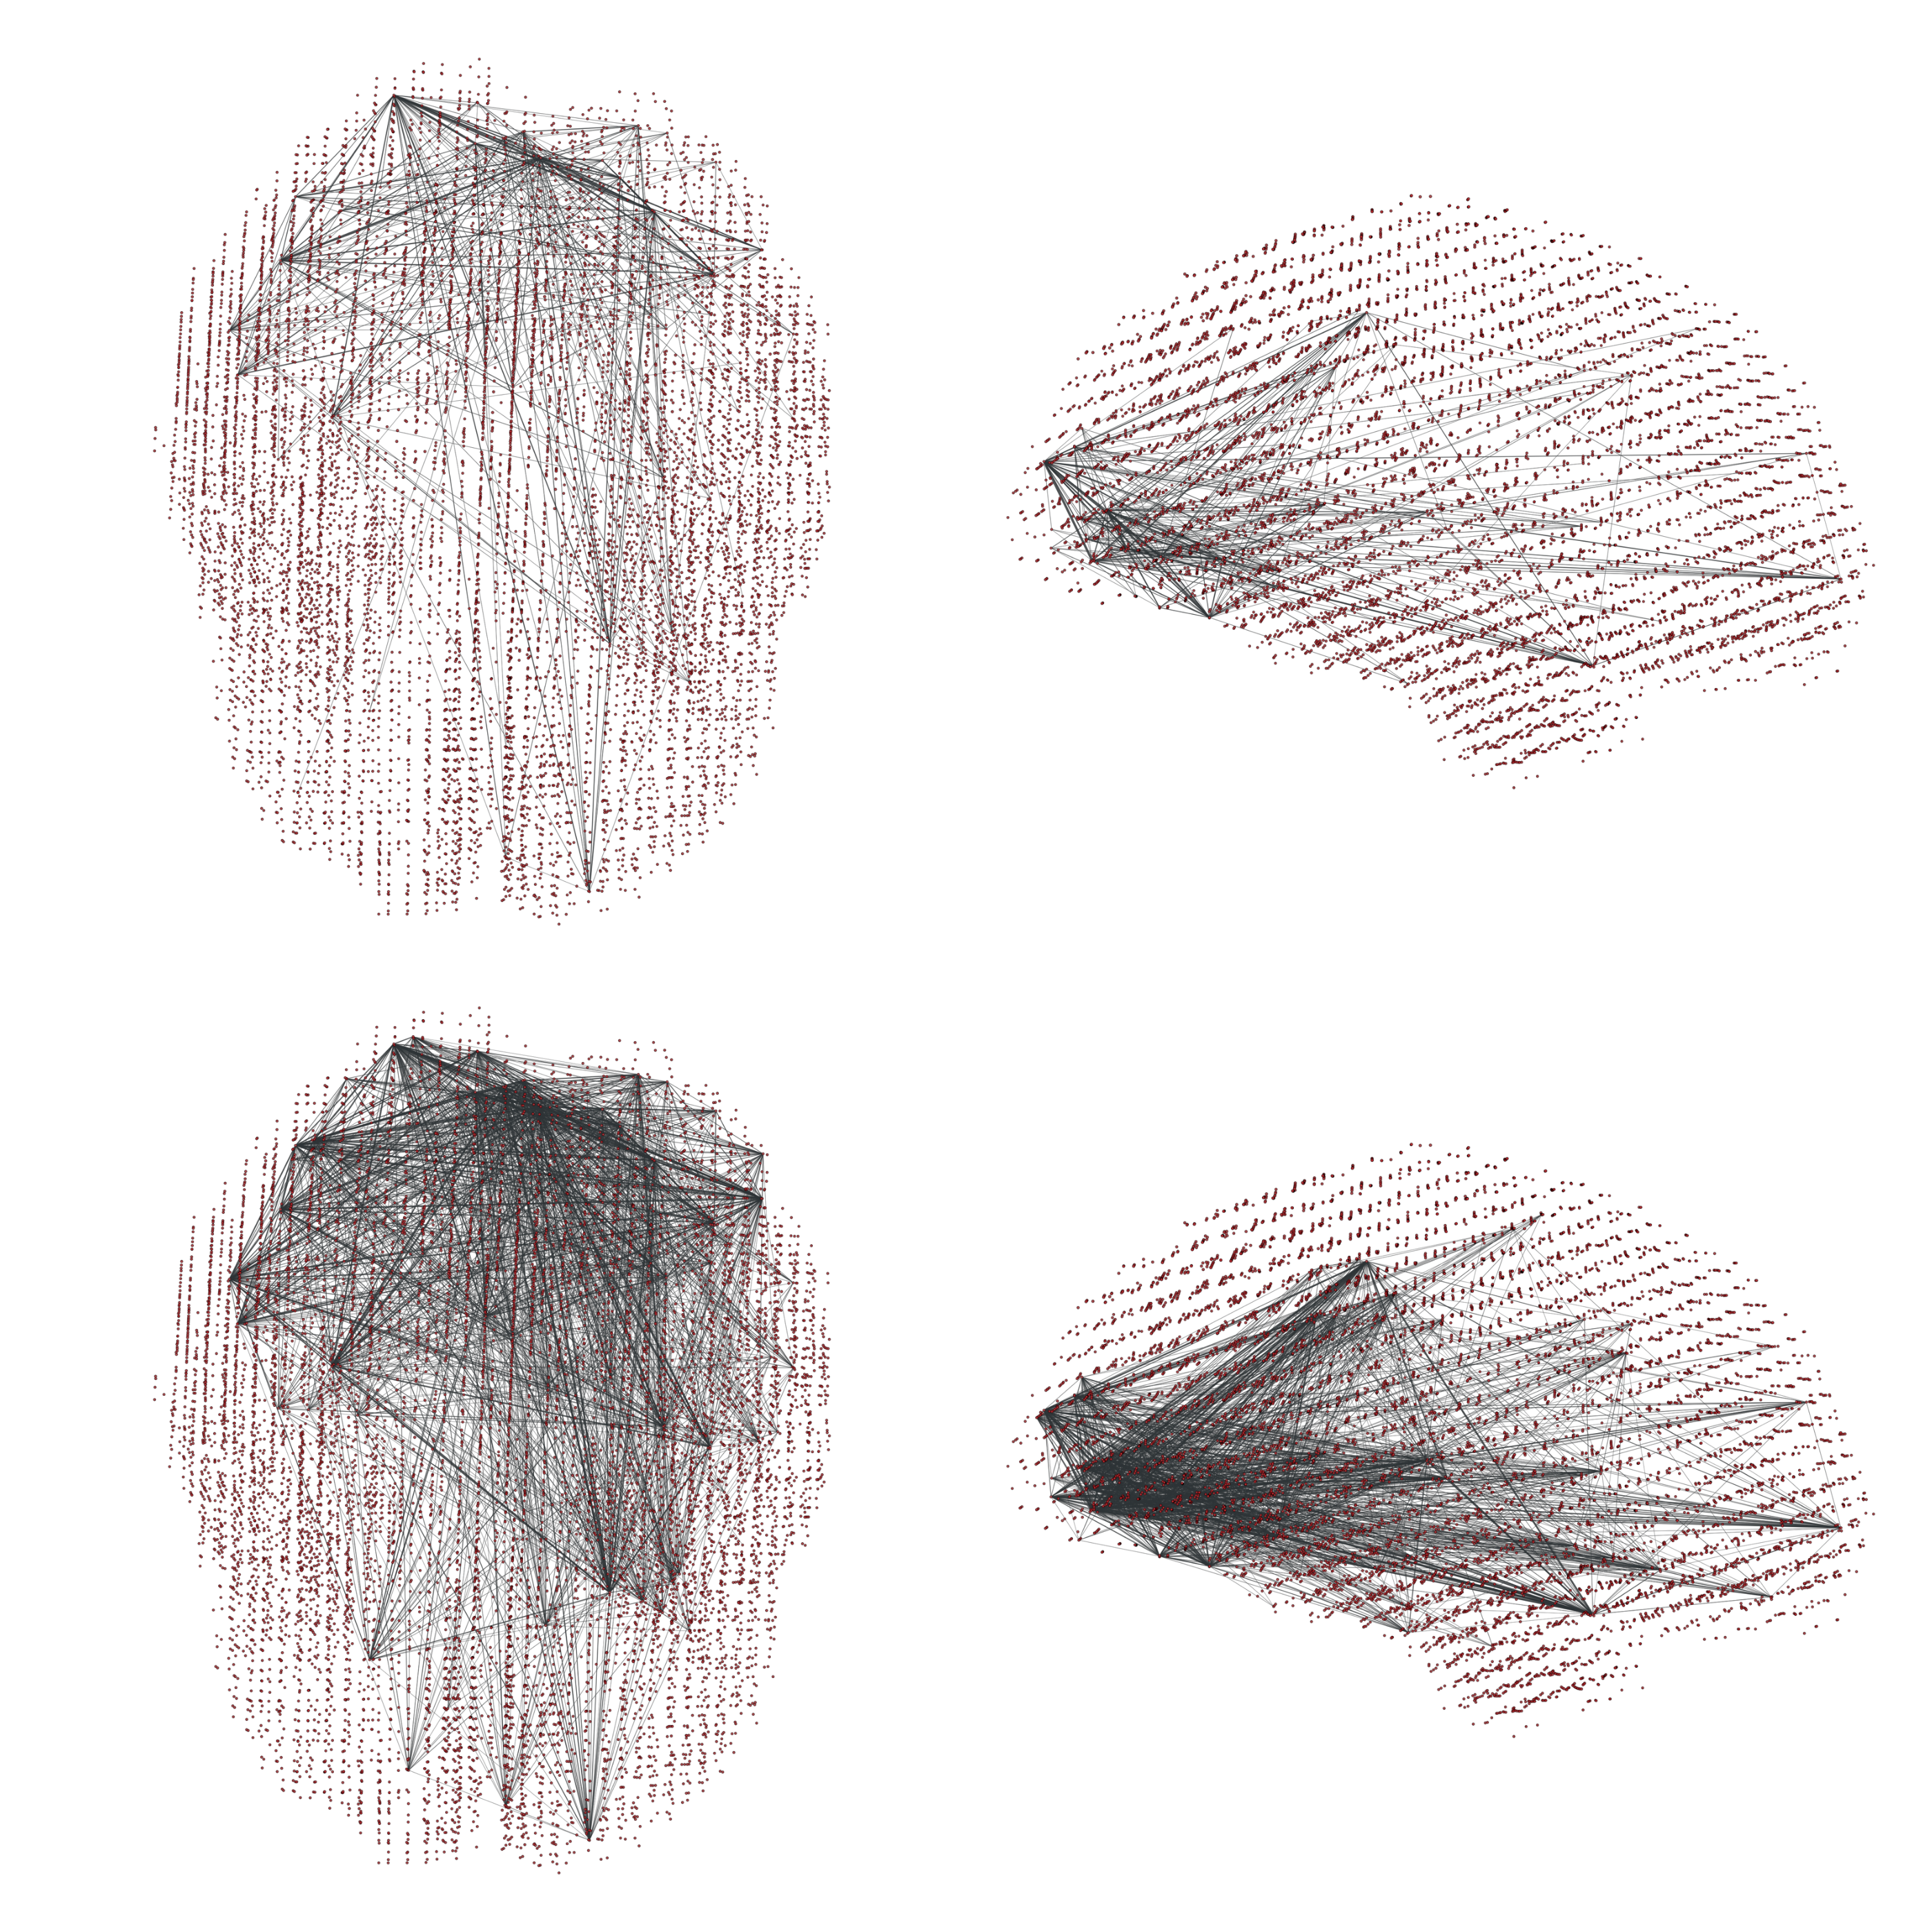
\includegraphics[width=0.48\textwidth]{figures/NW.png}%
\caption{Network plot showing the top edges from the $\bW$ matrix for the best-performing parameterization of group LASSO (top) and GrOWL (bottom) in one subject. The thickness of the edges is proportional to the edge weights.}
\label{fig.NW}
\end{figure}


\iffalse
\begin{figure*}[!t]
\centering
\includegraphics[width=0.75\textwidth]{figures/brain_final.png}%
\caption{Brain plots.}
\label{fig.brain}
\end{figure*}

\begin{figure}[!t]
    \centering
  \includegraphics[width=0.35\textwidth]{figures/Final_Error_Visual.png}
      
    \caption{Mean hold-out prediction error for group lasso and GrOWLs with real data.}
    \label{fig.error}
  \end{figure}



\fi



	\section{Conclusion}
%We have developed and demonstrated a new approach for whole-brain Representational Similarity Analysis called Network RSA (NRSA). Unlike traditional RSA methods that consider only specific regions of interest or spherical clusters of the cortex,  NRSA can discover arbitrarily structured brain networks (possibly widely distributed and non-local) that encode similarity information.  NRSA is posed as a sparsity-regularized multi-task regression problem. This allows us to effectively search over all subsets of voxels (not just localized clusters) to detect similarity-encoding networks.  We proposed a new sparsity regularizer for multi-task regression that is able to cope with strongly correlated covariates (voxels in the fMRI application), which can perform better than the conventional group lasso. named the GrOWL.  Experiments with real and synthetic datasets demonstrated the potential of our new approach.

We have developed and demonstrated a new approach for whole-brain Representational
Similarity Analysis called Network RSA (NRSA). Unlike traditional RSA methods that
consider only specific regions of interest or spherical clusters of the cortex,  NRSA can
discover arbitrarily structured brain networks (possibly widely distributed and non-local)
that encode similarity information.  NRSA is posed as a sparsity-regularized multi-task
regression problem. This allows us to effectively search over all subsets of voxels (not
just localized clusters) to detect similarity-encoding networks.  We further proposed a
new sparsity regularizer for multi-task regression, the GrOWL, that is able to cope with
strongly correlated covariates, a serious challenge for sparsity-based approaches to fMRI
analysis.

Our analysis of synthetic data generated from a neural network model of word-reading
showed that the GrOWL identifies signal-carrying features more consistently than group
lasso when signal is redundant; that the approach can discover different feature subsets
encoding different kinds of similarity structure; and that the weight matrix $\bW$ can be
used to uncover subnetworks of features that jointly work to encode such structure.
Analysis of visual similarity structure in fMRI data from a picture-viewing task further
established that the approach can be used to find cortical regions and subnetworks that
likewise express a target similarity structure. In future work these methods may be useful
for discovering such structure for cases where the interesting cortical regions and
networks have proven elusive.


\bibliographystyle{icml2016}
\bibliography{icml16_nrsa}


\end{document}


% This document was modified from the file originally made available by
% Pat Langley and Andrea Danyluk for ICML-2K. This version was
% created by Lise Getoor and Tobias Scheffer, it was slightly modified
% from the 2010 version by Thorsten Joachims & Johannes Fuernkranz,
% slightly modified from the 2009 version by Kiri Wagstaff and
% Sam Roweis's 2008 version, which is slightly modified from
% Prasad Tadepalli's 2007 version which is a lightly
% changed version of the previous year's version by Andrew Moore,
% which was in turn edited from those of Kristian Kersting and
% Codrina Lauth. Alex Smola contributed to the algorithmic style files.
